\scanpage{37}
% archive foliation: 36
\deleted{pour tout} posant $K^{(i)}=K\times_T T_i$, pour tt $T'$ sur $T_i$, le morphisme canonique
\[
H^q(K^{(i)}\otimes_{T_i}\unsure{T'_i|T'})\longleftarrow H^q(K^{(i)})\otimes_{T_i}T'
\]
soit un isomorphisme pour $|q|\leq N$.

Démonstration par récurrence noethérienne sur $T$, on est ramené à prouver qu'il existe un ouvert $U$ non vide de $T$ ayant la propriété des $T_i$, \inserted{$T$ étant supposé réduit.} Pour ceci, on \deleted{considère les \unsure{sous-faisceaux}} \inserted{choisit $U$ tel que les $B_i\otimes_TU$ \deleted{$\unsure{K_i}$} et $K_i$} \deleted{(cobords) $\times_TU$ \unsure{et les} soient $U$-plats pour $i$ \inserted{$|i|\leq N+1$} [$U$ étant pris avec la structure induite]} \unsure{donc} \unsure{sont} $U$-plats, pour $|i|\leq N+1$ ---

\margin{\diagram{\begin{tikzcd}[column sep=small,row sep=small]
K_{\unsure{i}}\arrow[r,"d_i"]&K_{i+1}\arrow[r,"d_{i+1}"]&K_{i+2}\\
&\unsure{H|B}_{i+1}&
\end{tikzcd}}}

\margin{\textcircled{b}\figure{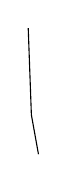
\begin{tikzpicture}\draw (0,0)--(.04,-1.1)--(.13,-1.6);\end{tikzpicture}}}
Soit $f:X-Y$ un $S$-morphisme de préschémas de type \unsure{finis}. Soit $A\subset\Phi(Y/S)$ une partie limitée, alors $f^*(A)$ et les $\operatorname{Tor}^{\underline O_Y}_{*}(A,\underline O_X)$ sont limités

Il y a intérêt à bloquer cette proposition avec la précédente, en \unsure{prenant} \deleted{\illegible{1}} $X$ et $Z$ sur $Y$, \deleted{et \illegible{1}} $A\subset\Phi(X/S)$, $B\subset\Phi(Y/S)$ et les $\operatorname{Tor}_i^{\underline O_Z}(A,B)$.
